\section{Manuale utente}
L'utente può interfacciarsi con l'applicazione tramite diverse schermate. Innanzitutto, e' possibile registrarsi creando un nuovo account o eventualmente eseguire direttamente il login. Per fare ciò sono state predisposte le due interfacce \ref{fig:login} e \ref{fig:signup}. Nel database reso a disposizione per la presentazione del progetto sono già inseriti 5 utenti (quelli generati dal mockup e l'admin generato in automatico). Per esempio è possibile accedere come utente normale usando:
\begin{itemize}
    \item username: mario@rossi.com
    \item password: mario
\end{itemize}
E come organizzatore usando:
\begin{itemize}
    \item username: giuseppe@verdi.com
    \item password: giuseppe
\end{itemize}
Eseguito l'accesso tramite le proprie credenziali utente, si viene reindirizzati alla schermata principale che mostra gli eventi disponibili \ref{fig:home}. In alto a sinistra è possibile accedere al proprio profilo \ref{fig:profile}, mentre tramite l'apposita icona si apre la sezione cerca \ref{fig:cerca}, da cui si possono cercare più rapidamente specifici eventi. La creazione di una nuova escursione è possibile solo se loggati come organizzatore e avviene facendo click sul bottone "nuova escursione", in quanto si verrà rimandati alla schermata  da cui inserire le informazioni del nuovo evento \ref{fig:new} (qualora l'utente sia un organizzatore). Inoltre, tramite la barra di navigazione è possibile accedere alla sezione dedicata ai consigliati \ref{fig:suggerimenti} ed alle iscrizioni \ref{fig:iscrizioni}, in cui vengono mostrati gli eventi ai quali si è iscritti. Infine, da da qualsiasi schermata è possibile accedere al profilo di ogni evento, nel quale vengono mostrate tutte le specifiche inserite
dall'utente organizzatore.
\begin{figure}[h!]
    \begin{center}
    \begin{multicols}{2}
        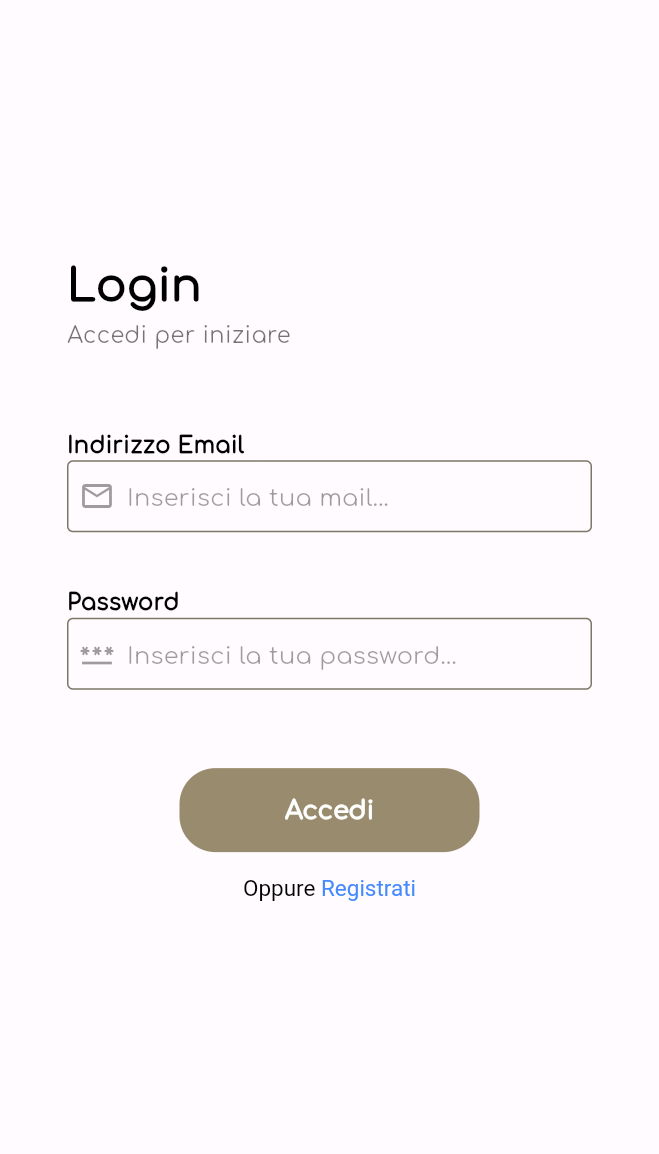
\includegraphics[width=0.55\linewidth]{Iterazione 4 finale/images/login.png}
        \caption{Login screen}\label{fig:login}
        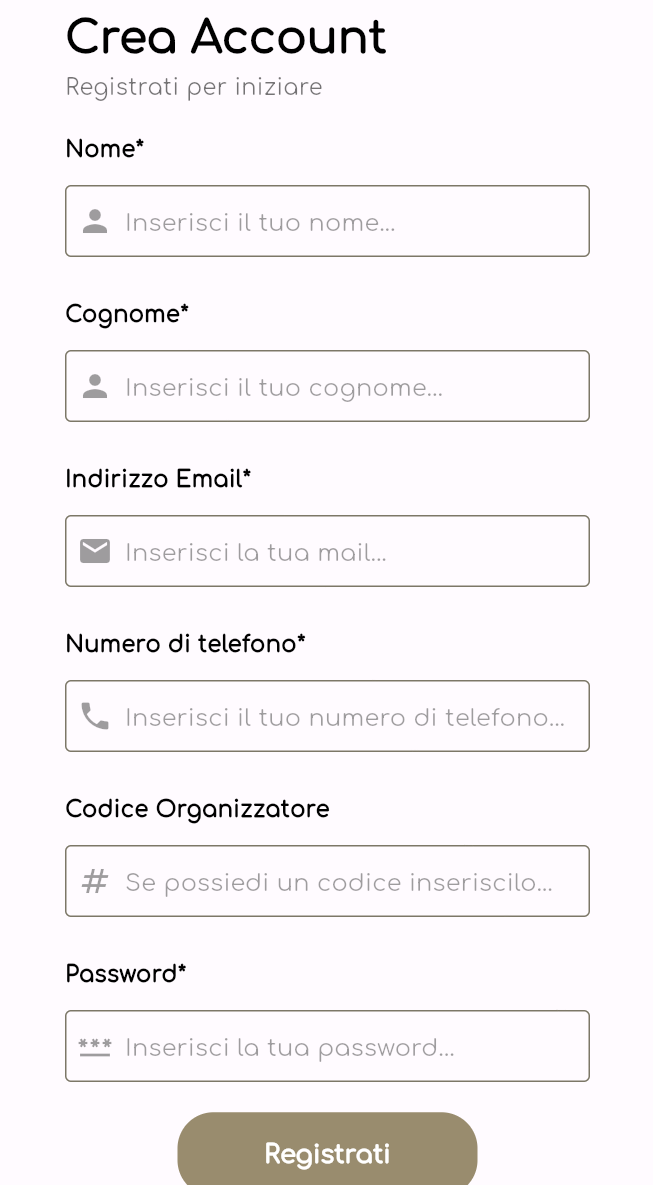
\includegraphics[width=0.55\linewidth]{Iterazione 4 finale/images/signup.png}
        \caption{Signup screen}\label{fig:signup}
    \end{multicols}
    \begin{multicols}{2}
        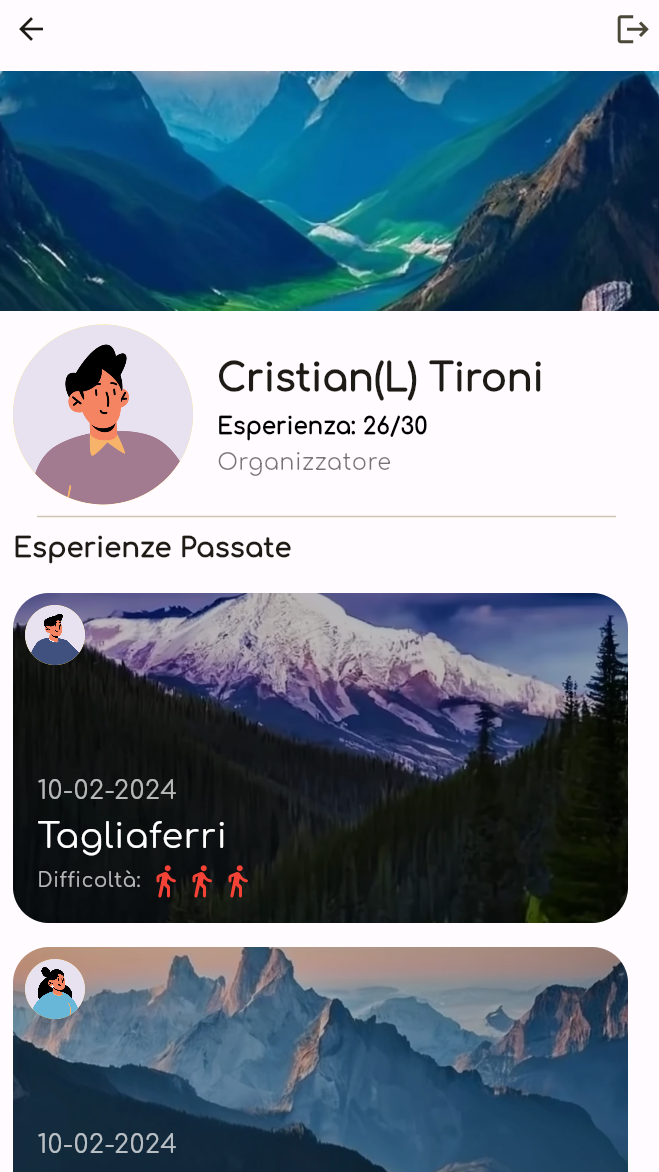
\includegraphics[width=0.55\linewidth]{Iterazione 4 finale/images/profile.png}
        \caption{Profilo utente}\label{fig:profile}
        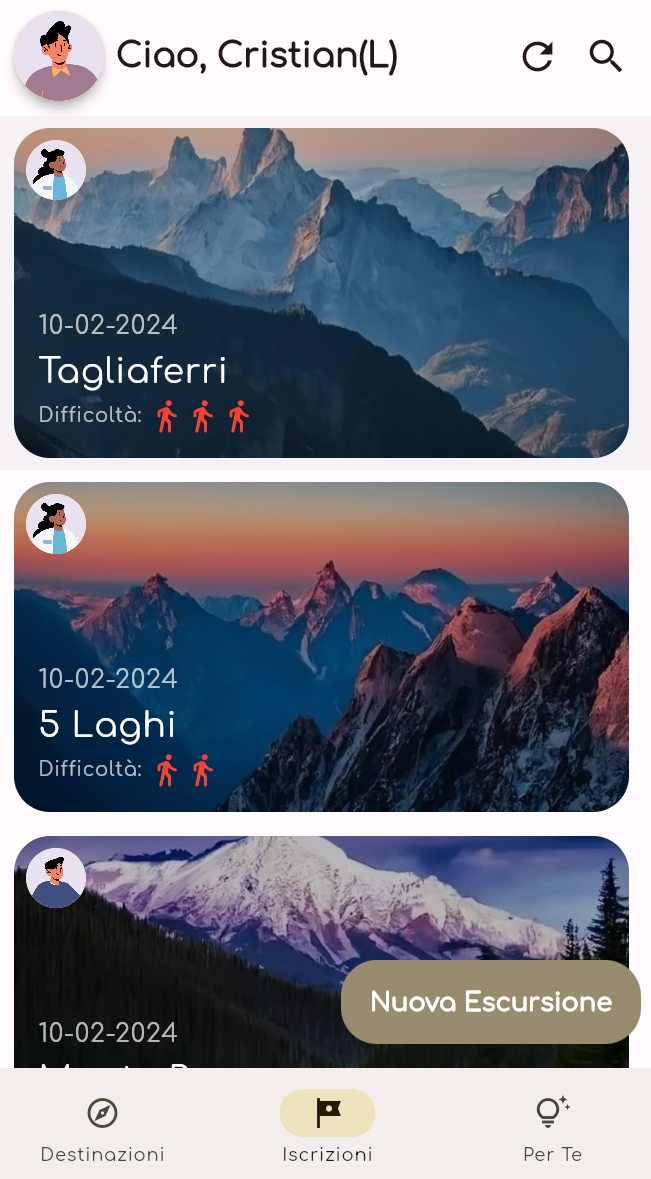
\includegraphics[width=0.55\linewidth]{Iterazione 4 finale/images/iscrizioni.png}
        \caption{Iscrizioni}\label{fig:iscrizioni}
    \end{multicols}
\end{center}
\end{figure} 
\begin{figure}[h!]
    \begin{center}
    \begin{multicols}{2}
        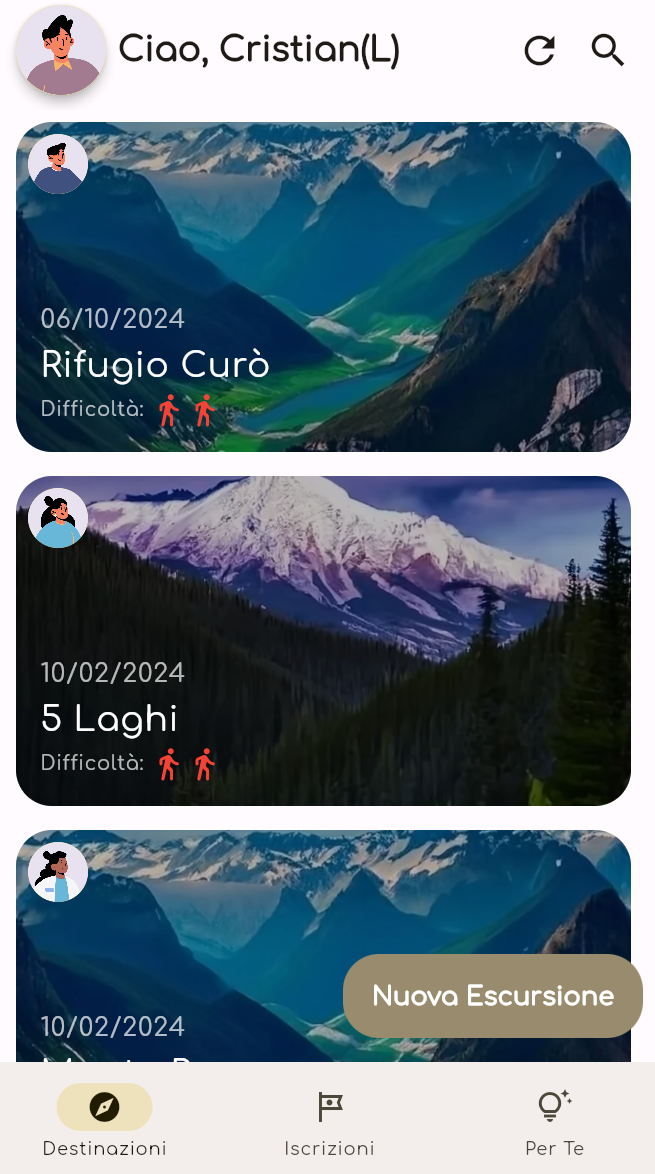
\includegraphics[width=0.55\linewidth]{Iterazione 4 finale/images/home.png}
        \caption{Homescreen}\label{fig:home}
        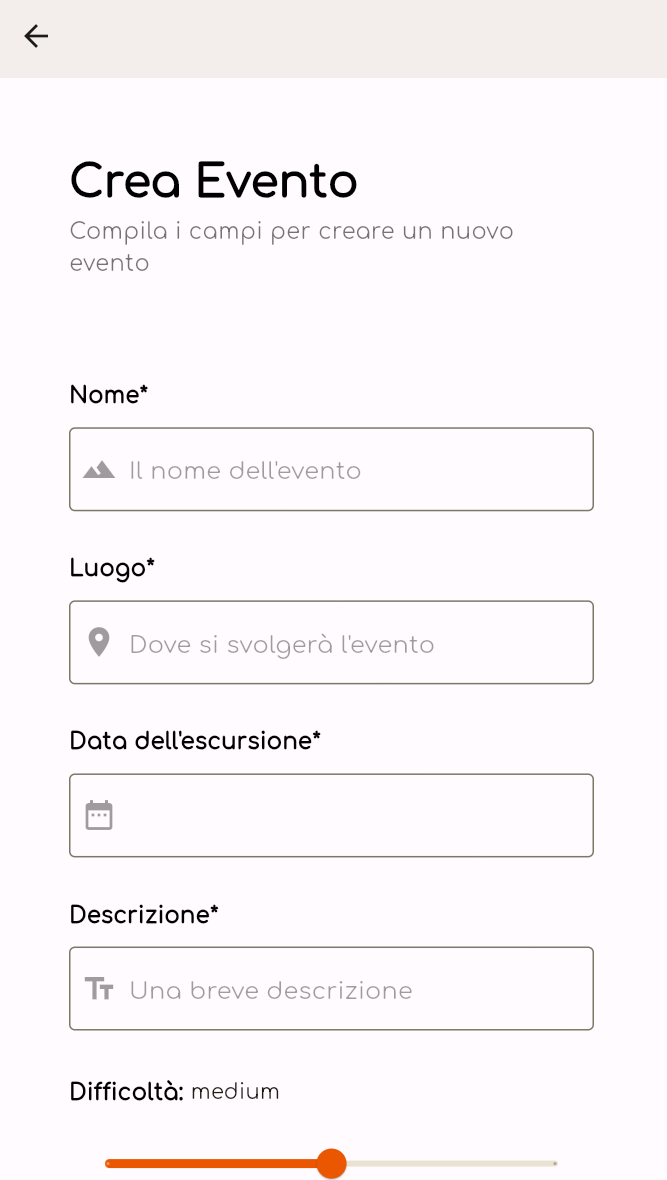
\includegraphics[width=0.55\linewidth]{Iterazione 4 finale/images/new evento.png}
        \caption{New evento}\label{fig:new}
    \end{multicols}
    \begin{multicols}{2}
        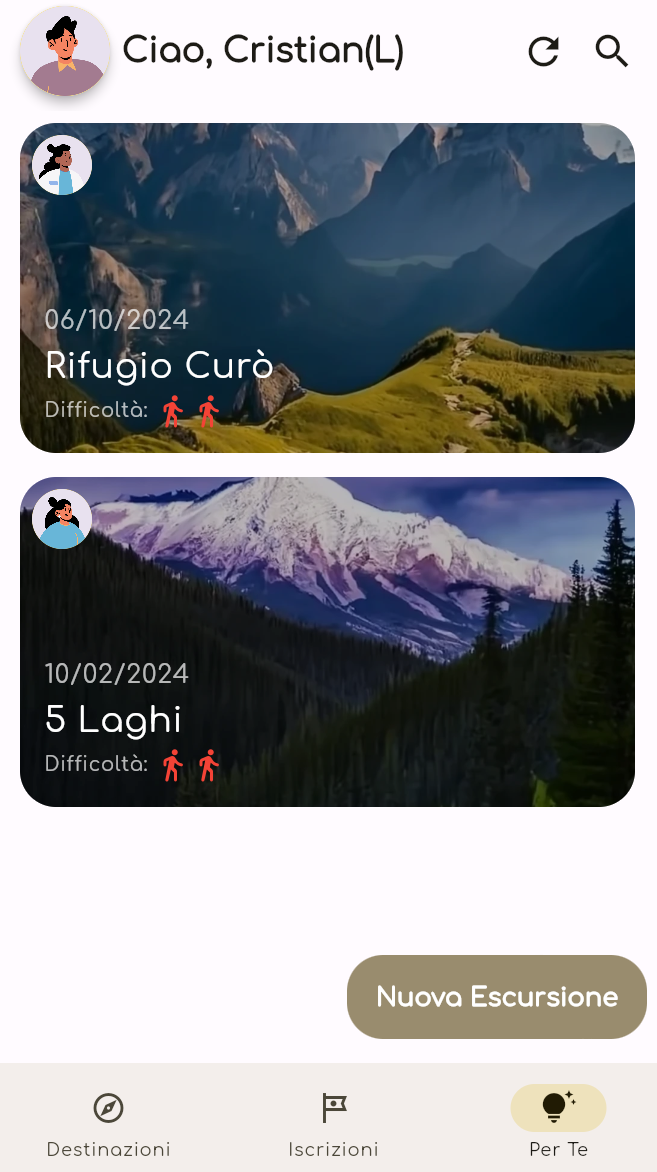
\includegraphics[width=0.55\linewidth]{Iterazione 4 finale/images/suggerimenti.png}
        \caption{Suggerimenti}\label{fig:suggerimenti}
        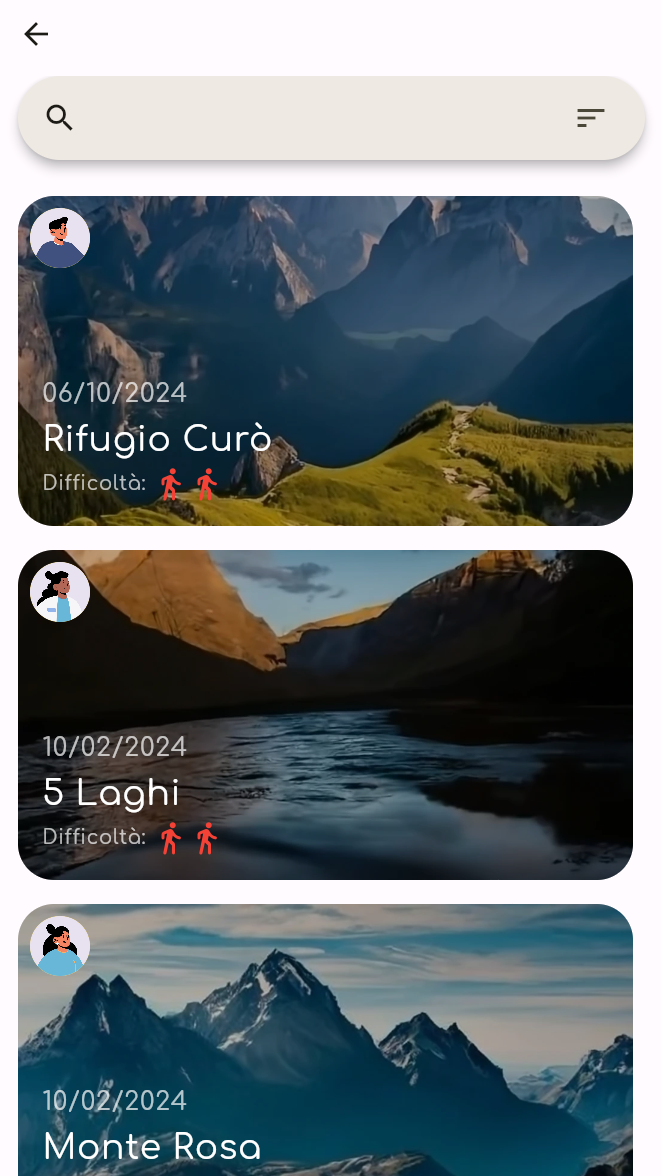
\includegraphics[width=0.55\linewidth]{Iterazione 4 finale/images/cerca.png}
        \caption{Cerca}\label{fig:cerca}
    \end{multicols}
\end{center}
\end{figure} 